 
\documentclass[12pt,a4paper,fleqn]{tufte-handout}     
\usepackage{graphicx}     
\usepackage{morefloats}     
\usepackage{amsmath}     
\usepackage{amssymb}     
\usepackage{rotating}     
% mcode options for matlab code insertion bw (for printing), numbered (line numbers), framed (frame around code blocks), useliterate (convert Matlab expressions to Latex ones), autolinebreaks (automatic code wraping, use it with caution     
\usepackage[literate]{mcode}     
\graphicspath{{figures/}{tex/}{../figures/}{../../}{../}}      
\title{sceneSvm}     
\author{ Grégoire Lafay }     
 
\begin{document}     
 
\maketitle     
 
% Please use this file to document your experiment     
% You can compile the report by setting the option 'report' as detailed in your expLanes configuration file.     
 
 
 
 
 
 
\begin{table}   
\begin{center}   
\scriptsize   
\setlength{\tabcolsep}{.16667em}   
\begin{tabular}{lllllc}   
features & kernel & cut & distance & select & accuracy \\   
\hline   
mfcc & objectBased & 0.02 & closest & 10 & 0.49$\pm$0.07 \\   
mfcc & objectBased & 0.02 & closest & 20 & 0.50$\pm$0.09 \\   
mfcc & objectBased & 0.02 & closest & 30 & 0.46$\pm$0.10 \\   
mfcc & objectBased & 0.02 & closest & 40 & 0.49$\pm$0.09 \\   
mfcc & objectBased & 0.02 & emd & 10 & 0.52$\pm$0.14 \\   
mfcc & objectBased & 0.02 & emd & 20 & 0.53$\pm$0.14 \\   
mfcc & objectBased & 0.02 & emd & 30 & \textbf{0.54$\pm$0.16} \\   
mfcc & objectBased & 0.02 & emd & 40 & 0.54$\pm$0.12 \\   
mfcc & objectBased & 0.04 & closest & 10 & 0.50$\pm$0.08 \\   
mfcc & objectBased & 0.04 & closest & 20 & 0.46$\pm$0.07 \\   
mfcc & objectBased & 0.04 & closest & 30 & 0.46$\pm$0.10 \\   
mfcc & objectBased & 0.04 & closest & 40 & 0.51$\pm$0.08 \\   
mfcc & objectBased & 0.04 & emd & 10 & 0.53$\pm$0.12 \\   
mfcc & objectBased & 0.04 & emd & 20 & 0.54$\pm$0.13 \\   
mfcc & objectBased & 0.04 & emd & 30 & 0.54$\pm$0.14 \\   
mfcc & objectBased & 0.04 & emd & 40 & 0.55$\pm$0.13 \\   
mfcc & objectBased & 0.08 & closest & 10 & 0.50$\pm$0.06 \\   
mfcc & objectBased & 0.08 & closest & 20 & 0.45$\pm$0.07 \\   
mfcc & objectBased & 0.08 & closest & 30 & 0.43$\pm$0.06 \\   
mfcc & objectBased & 0.08 & closest & 40 & 0.49$\pm$0.11 \\   
mfcc & objectBased & 0.08 & emd & 10 & 0.52$\pm$0.12 \\   
mfcc & objectBased & 0.08 & emd & 20 & 0.56$\pm$0.12 \\   
mfcc & objectBased & 0.08 & emd & 30 & 0.53$\pm$0.14 \\   
mfcc & objectBased & 0.08 & emd & 40 & 0.55$\pm$0.11 \\   
mfcc & objectBased & 0.10 & closest & 10 & 0.49$\pm$0.07 \\   
mfcc & objectBased & 0.10 & closest & 20 & 0.44$\pm$0.07 \\   
mfcc & objectBased & 0.10 & closest & 30 & 0.46$\pm$0.07 \\   
mfcc & objectBased & 0.10 & closest & 40 & 0.48$\pm$0.10 \\   
mfcc & objectBased & 0.10 & emd & 10 & 0.52$\pm$0.12 \\   
mfcc & objectBased & 0.10 & emd & 20 & 0.54$\pm$0.13 \\   
mfcc & objectBased & 0.10 & emd & 30 & 0.54$\pm$0.13 \\   
mfcc & objectBased & 0.10 & emd & 40 & 0.55$\pm$0.11 \\   
scatteringV & objectBased & 0.02 & closest & 10 & \textbf{0.71$\pm$0.08} \\   
scatteringV & objectBased & 0.02 & closest & 20 & \textbf{\textcolor{red}{0.72$\pm$0.08}} \\   
scatteringV & objectBased & 0.02 & closest & 30 & \textbf{0.68$\pm$0.10} \\   
scatteringV & objectBased & 0.02 & closest & 40 & \textbf{0.69$\pm$0.08} \\   
scatteringV & objectBased & 0.02 & emd & 10 & \textbf{0.65$\pm$0.11} \\   
scatteringV & objectBased & 0.02 & emd & 20 & \textbf{0.67$\pm$0.13} \\   
scatteringV & objectBased & 0.02 & emd & 30 & \textbf{0.66$\pm$0.11} \\   
scatteringV & objectBased & 0.02 & emd & 40 & \textbf{0.65$\pm$0.13} \\   
scatteringV & objectBased & 0.04 & closest & 10 & \textbf{\textcolor{red}{0.72$\pm$0.09}} \\   
scatteringV & objectBased & 0.04 & closest & 20 & \textbf{0.70$\pm$0.10} \\   
scatteringV & objectBased & 0.04 & closest & 30 & \textbf{0.68$\pm$0.08} \\   
scatteringV & objectBased & 0.04 & closest & 40 & \textbf{0.68$\pm$0.08} \\   
scatteringV & objectBased & 0.04 & emd & 10 & \textbf{0.63$\pm$0.13} \\   
scatteringV & objectBased & 0.04 & emd & 20 & \textbf{0.65$\pm$0.13} \\   
scatteringV & objectBased & 0.04 & emd & 30 & \textbf{0.65$\pm$0.13} \\   
scatteringV & objectBased & 0.04 & emd & 40 & \textbf{0.65$\pm$0.13} \\   
scatteringV & objectBased & 0.08 & closest & 10 & \textbf{0.71$\pm$0.14} \\   
scatteringV & objectBased & 0.08 & closest & 20 & \textbf{0.69$\pm$0.13} \\   
scatteringV & objectBased & 0.08 & closest & 30 & \textbf{0.68$\pm$0.09} \\   
scatteringV & objectBased & 0.08 & closest & 40 & \textbf{0.68$\pm$0.07} \\   
scatteringV & objectBased & 0.08 & emd & 10 & \textbf{0.63$\pm$0.10} \\   
scatteringV & objectBased & 0.08 & emd & 20 & \textbf{0.65$\pm$0.13} \\   
scatteringV & objectBased & 0.08 & emd & 30 & \textbf{0.63$\pm$0.13} \\   
scatteringV & objectBased & 0.08 & emd & 40 & \textbf{0.63$\pm$0.13} \\   
scatteringV & objectBased & 0.10 & closest & 10 & \textbf{0.70$\pm$0.14} \\   
scatteringV & objectBased & 0.10 & closest & 20 & \textbf{0.69$\pm$0.13} \\   
scatteringV & objectBased & 0.10 & closest & 30 & \textbf{0.67$\pm$0.10} \\   
scatteringV & objectBased & 0.10 & closest & 40 & \textbf{0.68$\pm$0.07} \\   
scatteringV & objectBased & 0.10 & emd & 10 & \textbf{0.63$\pm$0.13} \\   
scatteringV & objectBased & 0.10 & emd & 20 & \textbf{0.63$\pm$0.13} \\   
scatteringV & objectBased & 0.10 & emd & 30 & \textbf{0.63$\pm$0.13} \\   
scatteringV & objectBased & 0.10 & emd & 40 & \textbf{0.63$\pm$0.13} \\   
mfcc & baseline & 0.02 &  &  & 0.46$\pm$0.13 \\   
mfcc & baseline & 0.04 &  &  & 0.48$\pm$0.10 \\   
mfcc & baseline & 0.08 &  &  & 0.47$\pm$0.14 \\   
mfcc & baseline & 0.10 &  &  & 0.48$\pm$0.13 \\   
scatteringV & baseline & 0.02 &  &  & \textbf{0.59$\pm$0.14} \\   
scatteringV & baseline & 0.04 &  &  & \textbf{0.61$\pm$0.14} \\   
scatteringV & baseline & 0.08 &  &  & \textbf{0.62$\pm$0.14} \\   
scatteringV & baseline & 0.10 &  &  & \textbf{0.61$\pm$0.14} \\   
\end{tabular}   
\end{center}   
\caption{set: train}   
\label{settr}   
\end{table}   
 
 
\begin{center}  
\begin{figure}  
\centering  
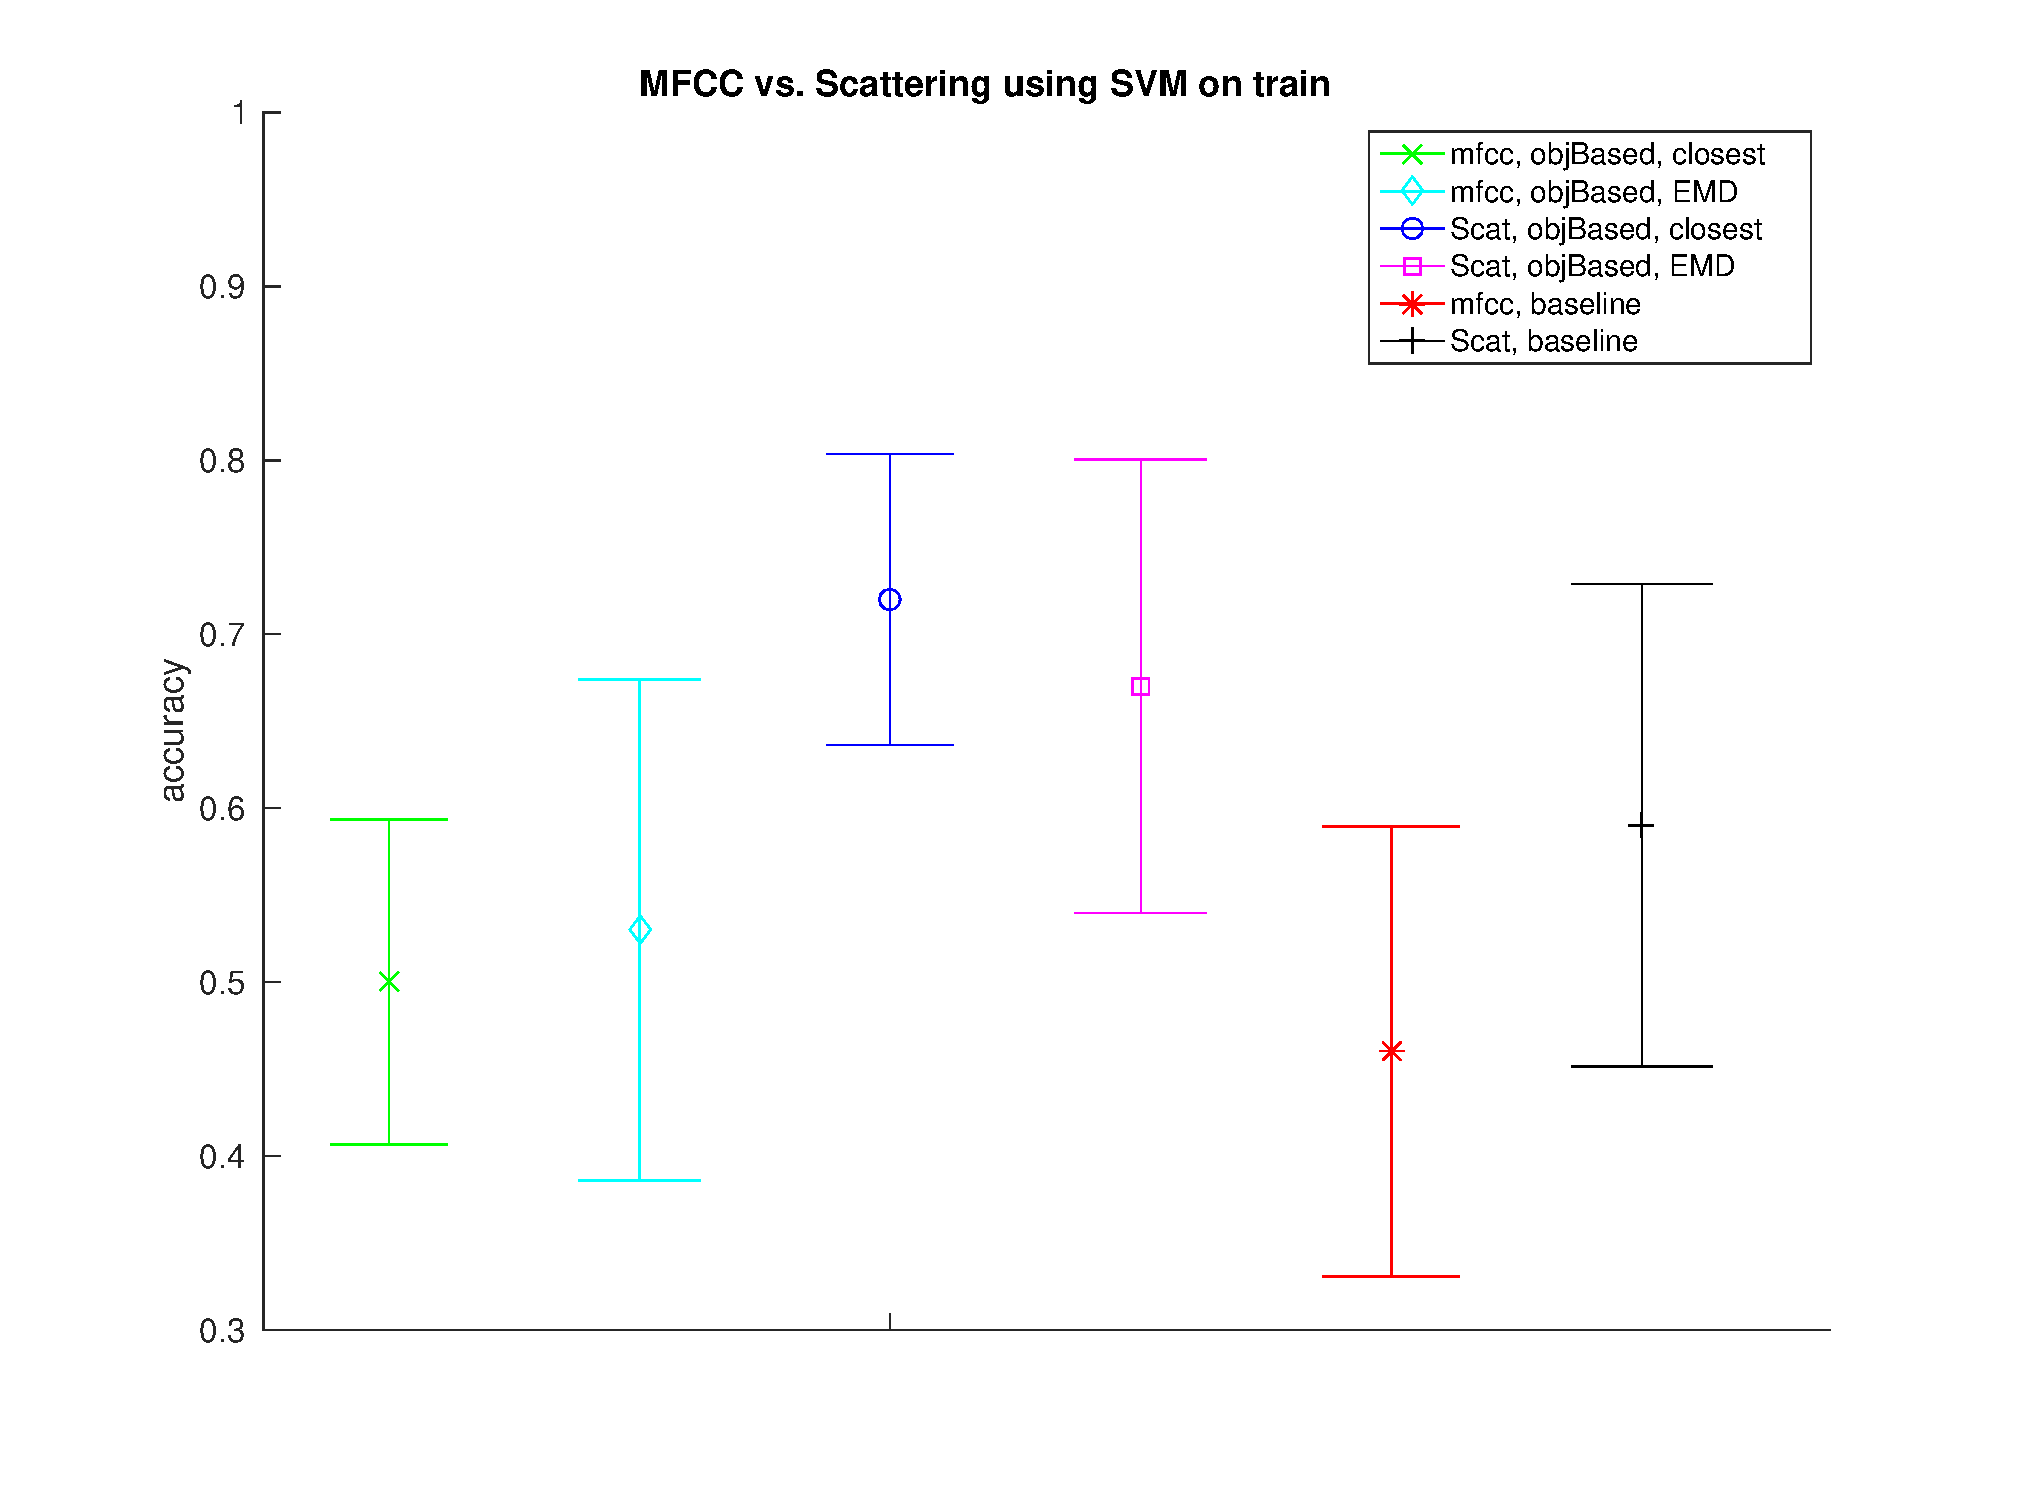
\includegraphics[width=\textwidth,height=0.8\textheight,keepaspectratio]{./figures/Fig5.pdf}  
\caption{cut: 0.02, set: train, select: 20}  
\label{cut0.02SettrSel20}  
\end{figure}  
\end{center}  
 
 
  
\begin{center} 
\begin{figure} 
\centering 
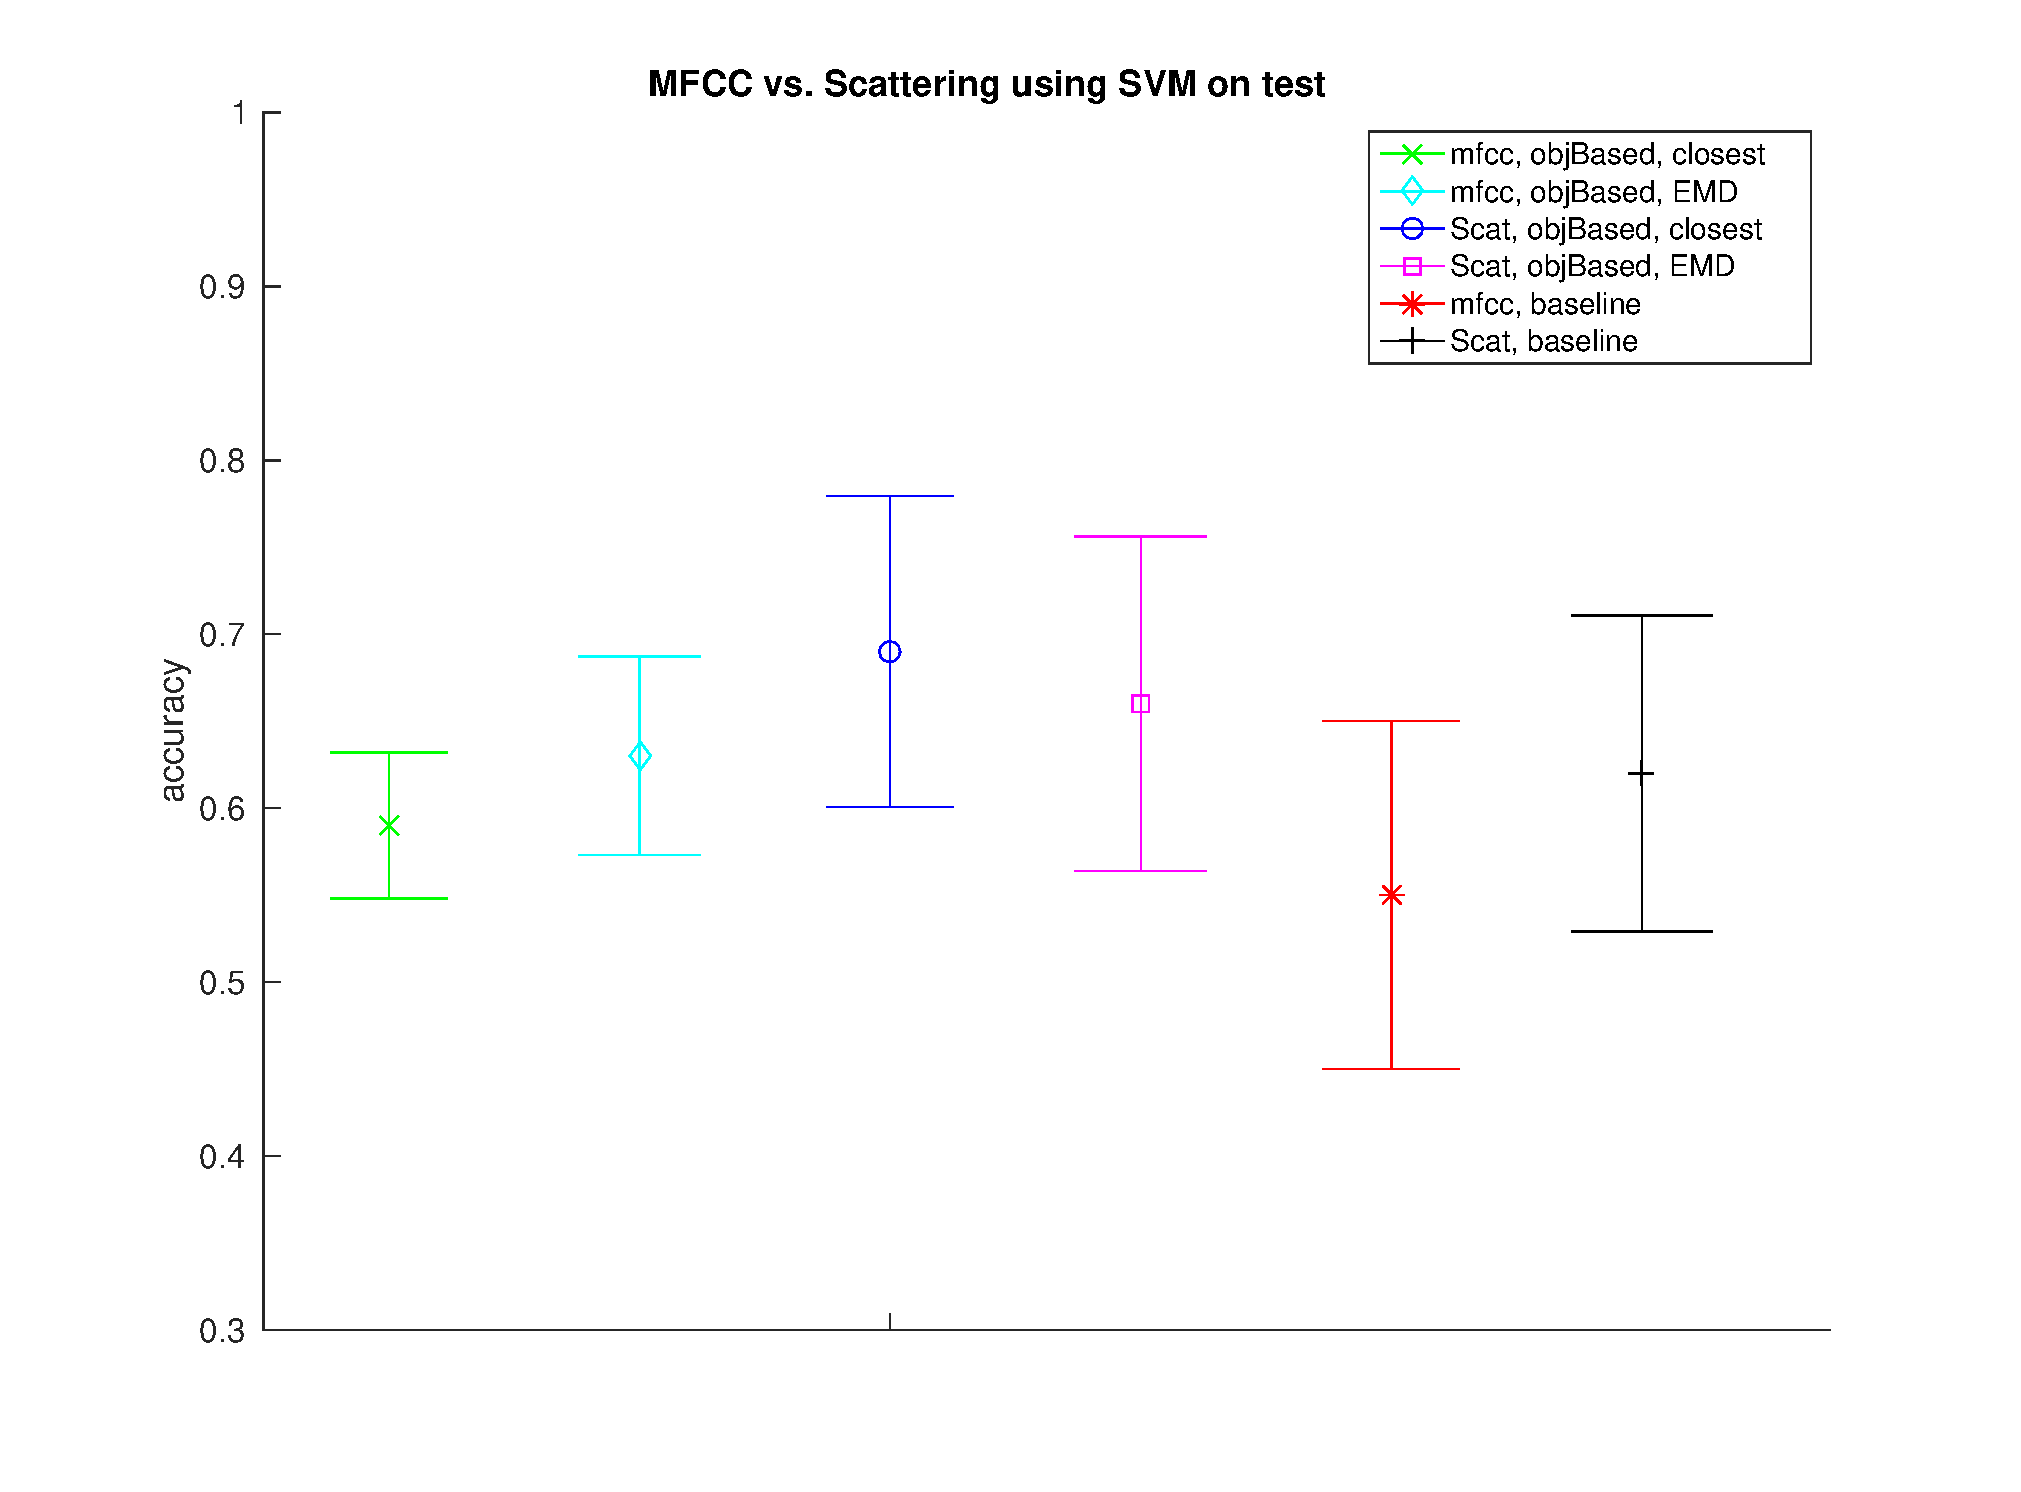
\includegraphics[width=\textwidth,height=0.8\textheight,keepaspectratio]{./figures/Fig6.pdf} 
\caption{cut: 0.02, set: test, select: 20} 
\label{cut0.02SetteSel20} 
\end{figure} 
\end{center} 
  
  
  
 
  
  
\begin{table} 
\begin{center} 
\scriptsize 
 \setlength{\tabcolsep}{.16667em} 
\begin{tabular}{lllllc} 
features & kernel & cut & distance & select & accuracy \\ 
\hline 
mfcc & objectBased & 0.02 & closest & 10 & 0.49$\pm$0.07 \\ 
mfcc & objectBased & 0.02 & closest & 20 & 0.50$\pm$0.09 \\ 
mfcc & objectBased & 0.02 & closest & 30 & 0.46$\pm$0.10 \\ 
mfcc & objectBased & 0.02 & closest & 40 & 0.49$\pm$0.09 \\ 
mfcc & objectBased & 0.02 & emd & 10 & 0.52$\pm$0.14 \\ 
mfcc & objectBased & 0.02 & emd & 20 & 0.53$\pm$0.14 \\ 
mfcc & objectBased & 0.02 & emd & 30 & \textbf{0.54$\pm$0.16} \\ 
mfcc & objectBased & 0.02 & emd & 40 & 0.54$\pm$0.12 \\ 
mfcc & objectBased & 0.04 & closest & 10 & 0.50$\pm$0.08 \\ 
mfcc & objectBased & 0.04 & closest & 20 & 0.46$\pm$0.07 \\ 
mfcc & objectBased & 0.04 & closest & 30 & 0.46$\pm$0.10 \\ 
mfcc & objectBased & 0.04 & closest & 40 & 0.51$\pm$0.08 \\ 
mfcc & objectBased & 0.04 & emd & 10 & 0.53$\pm$0.12 \\ 
mfcc & objectBased & 0.04 & emd & 20 & 0.54$\pm$0.13 \\ 
mfcc & objectBased & 0.04 & emd & 30 & 0.54$\pm$0.14 \\ 
mfcc & objectBased & 0.04 & emd & 40 & 0.55$\pm$0.13 \\ 
mfcc & objectBased & 0.08 & closest & 10 & 0.50$\pm$0.06 \\ 
mfcc & objectBased & 0.08 & closest & 20 & 0.45$\pm$0.07 \\ 
mfcc & objectBased & 0.08 & closest & 30 & 0.43$\pm$0.06 \\ 
mfcc & objectBased & 0.08 & closest & 40 & 0.49$\pm$0.11 \\ 
mfcc & objectBased & 0.08 & emd & 10 & 0.52$\pm$0.12 \\ 
mfcc & objectBased & 0.08 & emd & 20 & 0.56$\pm$0.12 \\ 
mfcc & objectBased & 0.08 & emd & 30 & 0.53$\pm$0.14 \\ 
mfcc & objectBased & 0.08 & emd & 40 & 0.55$\pm$0.11 \\ 
mfcc & objectBased & 0.10 & closest & 10 & 0.49$\pm$0.07 \\ 
mfcc & objectBased & 0.10 & closest & 20 & 0.44$\pm$0.07 \\ 
mfcc & objectBased & 0.10 & closest & 30 & 0.46$\pm$0.07 \\ 
mfcc & objectBased & 0.10 & closest & 40 & 0.48$\pm$0.10 \\ 
mfcc & objectBased & 0.10 & emd & 10 & 0.52$\pm$0.12 \\ 
mfcc & objectBased & 0.10 & emd & 20 & 0.54$\pm$0.13 \\ 
mfcc & objectBased & 0.10 & emd & 30 & 0.54$\pm$0.13 \\ 
mfcc & objectBased & 0.10 & emd & 40 & 0.55$\pm$0.11 \\ 
scatteringV & objectBased & 0.02 & closest & 10 & \textbf{0.71$\pm$0.08} \\ 
scatteringV & objectBased & 0.02 & closest & 20 & \textbf{\textcolor{red}{0.72$\pm$0.08}} \\ 
scatteringV & objectBased & 0.02 & closest & 30 & \textbf{0.68$\pm$0.10} \\ 
scatteringV & objectBased & 0.02 & closest & 40 & \textbf{0.69$\pm$0.08} \\ 
scatteringV & objectBased & 0.02 & emd & 10 & \textbf{0.65$\pm$0.11} \\ 
scatteringV & objectBased & 0.02 & emd & 20 & \textbf{0.67$\pm$0.13} \\ 
scatteringV & objectBased & 0.02 & emd & 30 & \textbf{0.66$\pm$0.11} \\ 
scatteringV & objectBased & 0.02 & emd & 40 & \textbf{0.65$\pm$0.13} \\ 
scatteringV & objectBased & 0.04 & closest & 10 & \textbf{\textcolor{red}{0.72$\pm$0.09}} \\ 
scatteringV & objectBased & 0.04 & closest & 20 & \textbf{0.70$\pm$0.10} \\ 
scatteringV & objectBased & 0.04 & closest & 30 & \textbf{0.68$\pm$0.08} \\ 
scatteringV & objectBased & 0.04 & closest & 40 & \textbf{0.68$\pm$0.08} \\ 
scatteringV & objectBased & 0.04 & emd & 10 & \textbf{0.63$\pm$0.13} \\ 
scatteringV & objectBased & 0.04 & emd & 20 & \textbf{0.65$\pm$0.13} \\ 
scatteringV & objectBased & 0.04 & emd & 30 & \textbf{0.65$\pm$0.13} \\ 
scatteringV & objectBased & 0.04 & emd & 40 & \textbf{0.65$\pm$0.13} \\ 
scatteringV & objectBased & 0.08 & closest & 10 & \textbf{0.71$\pm$0.14} \\ 
scatteringV & objectBased & 0.08 & closest & 20 & \textbf{0.69$\pm$0.13} \\ 
scatteringV & objectBased & 0.08 & closest & 30 & \textbf{0.68$\pm$0.09} \\ 
scatteringV & objectBased & 0.08 & closest & 40 & \textbf{0.68$\pm$0.07} \\ 
scatteringV & objectBased & 0.08 & emd & 10 & \textbf{0.63$\pm$0.10} \\ 
scatteringV & objectBased & 0.08 & emd & 20 & \textbf{0.65$\pm$0.13} \\ 
scatteringV & objectBased & 0.08 & emd & 30 & \textbf{0.63$\pm$0.13} \\ 
scatteringV & objectBased & 0.08 & emd & 40 & \textbf{0.63$\pm$0.13} \\ 
scatteringV & objectBased & 0.10 & closest & 10 & \textbf{0.70$\pm$0.14} \\ 
scatteringV & objectBased & 0.10 & closest & 20 & \textbf{0.69$\pm$0.13} \\ 
scatteringV & objectBased & 0.10 & closest & 30 & \textbf{0.67$\pm$0.10} \\ 
scatteringV & objectBased & 0.10 & closest & 40 & \textbf{0.68$\pm$0.07} \\ 
scatteringV & objectBased & 0.10 & emd & 10 & \textbf{0.63$\pm$0.13} \\ 
scatteringV & objectBased & 0.10 & emd & 20 & \textbf{0.63$\pm$0.13} \\ 
scatteringV & objectBased & 0.10 & emd & 30 & \textbf{0.63$\pm$0.13} \\ 
scatteringV & objectBased & 0.10 & emd & 40 & \textbf{0.63$\pm$0.13} \\ 
mfcc & baseline & 0.02 &  &  & 0.46$\pm$0.13 \\ 
mfcc & baseline & 0.04 &  &  & 0.48$\pm$0.10 \\ 
mfcc & baseline & 0.08 &  &  & 0.47$\pm$0.14 \\ 
mfcc & baseline & 0.10 &  &  & 0.48$\pm$0.13 \\ 
scatteringV & baseline & 0.02 &  &  & \textbf{0.59$\pm$0.14} \\ 
scatteringV & baseline & 0.04 &  &  & \textbf{0.61$\pm$0.14} \\ 
scatteringV & baseline & 0.08 &  &  & \textbf{0.62$\pm$0.14} \\ 
scatteringV & baseline & 0.10 &  &  & \textbf{0.61$\pm$0.14} \\ 
\end{tabular} 
\end{center} 
\caption{set: train} 
\label{settr} 
\end{table} 
 
  
\begin{center} 
\begin{figure} 
\centering 
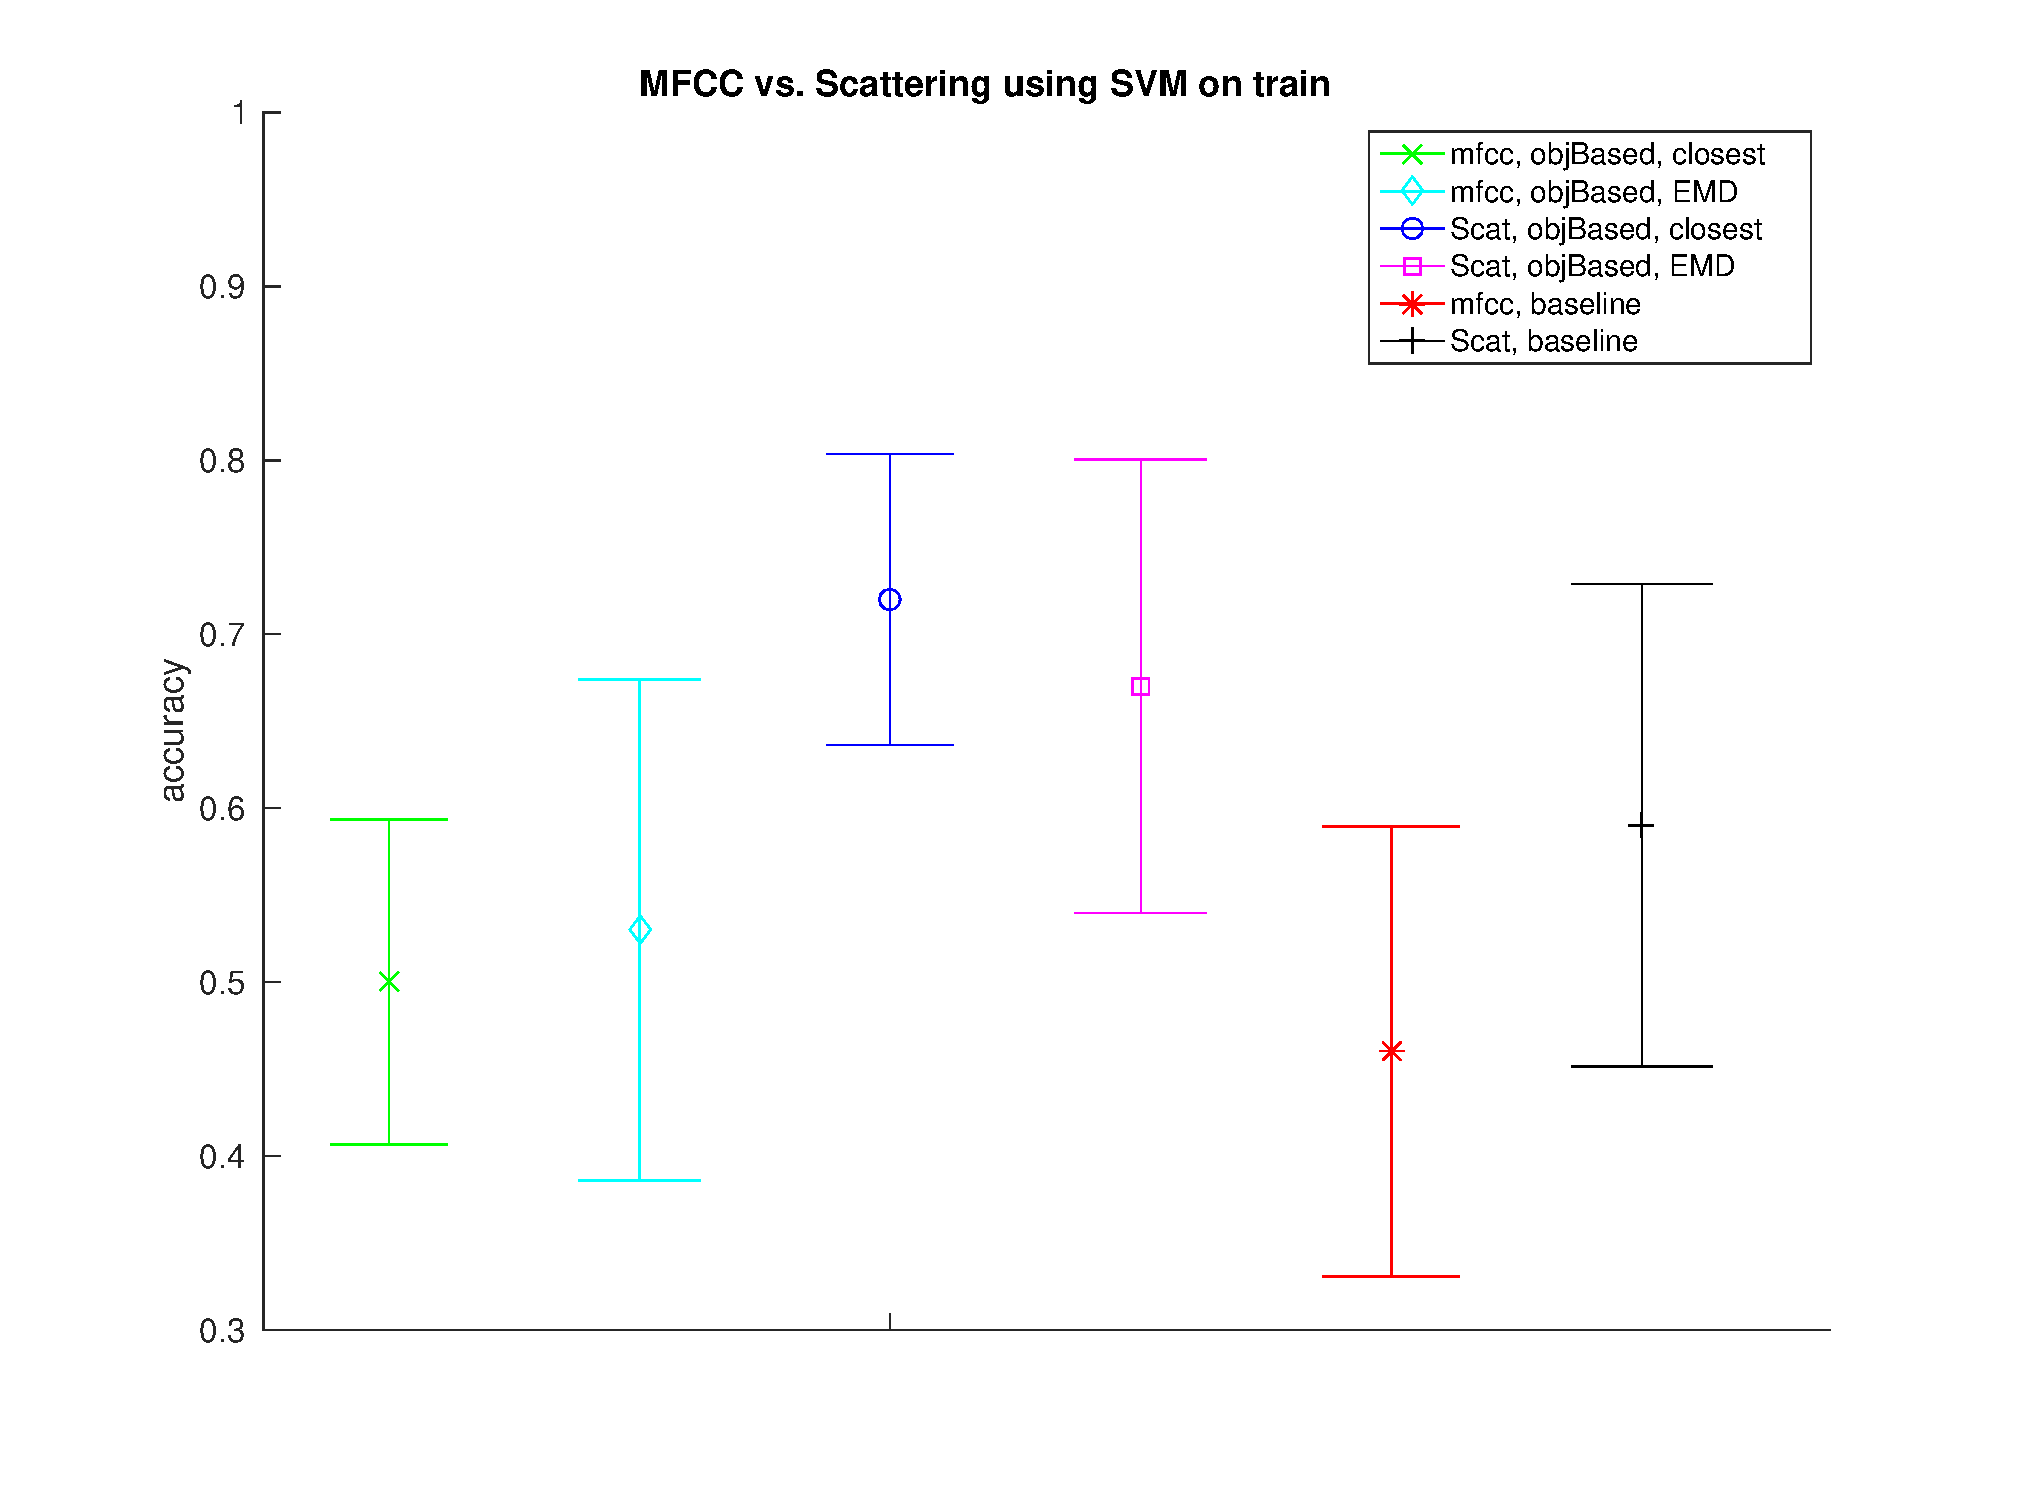
\includegraphics[width=\textwidth,height=0.8\textheight,keepaspectratio]{./figures/Fig5.pdf} 
\caption{cut: 0.02, set: train, select: 20} 
\label{cut0.02SettrSel20} 
\end{figure} 
\end{center} 
  
  
  
\begin{center} 
\begin{figure} 
\centering 
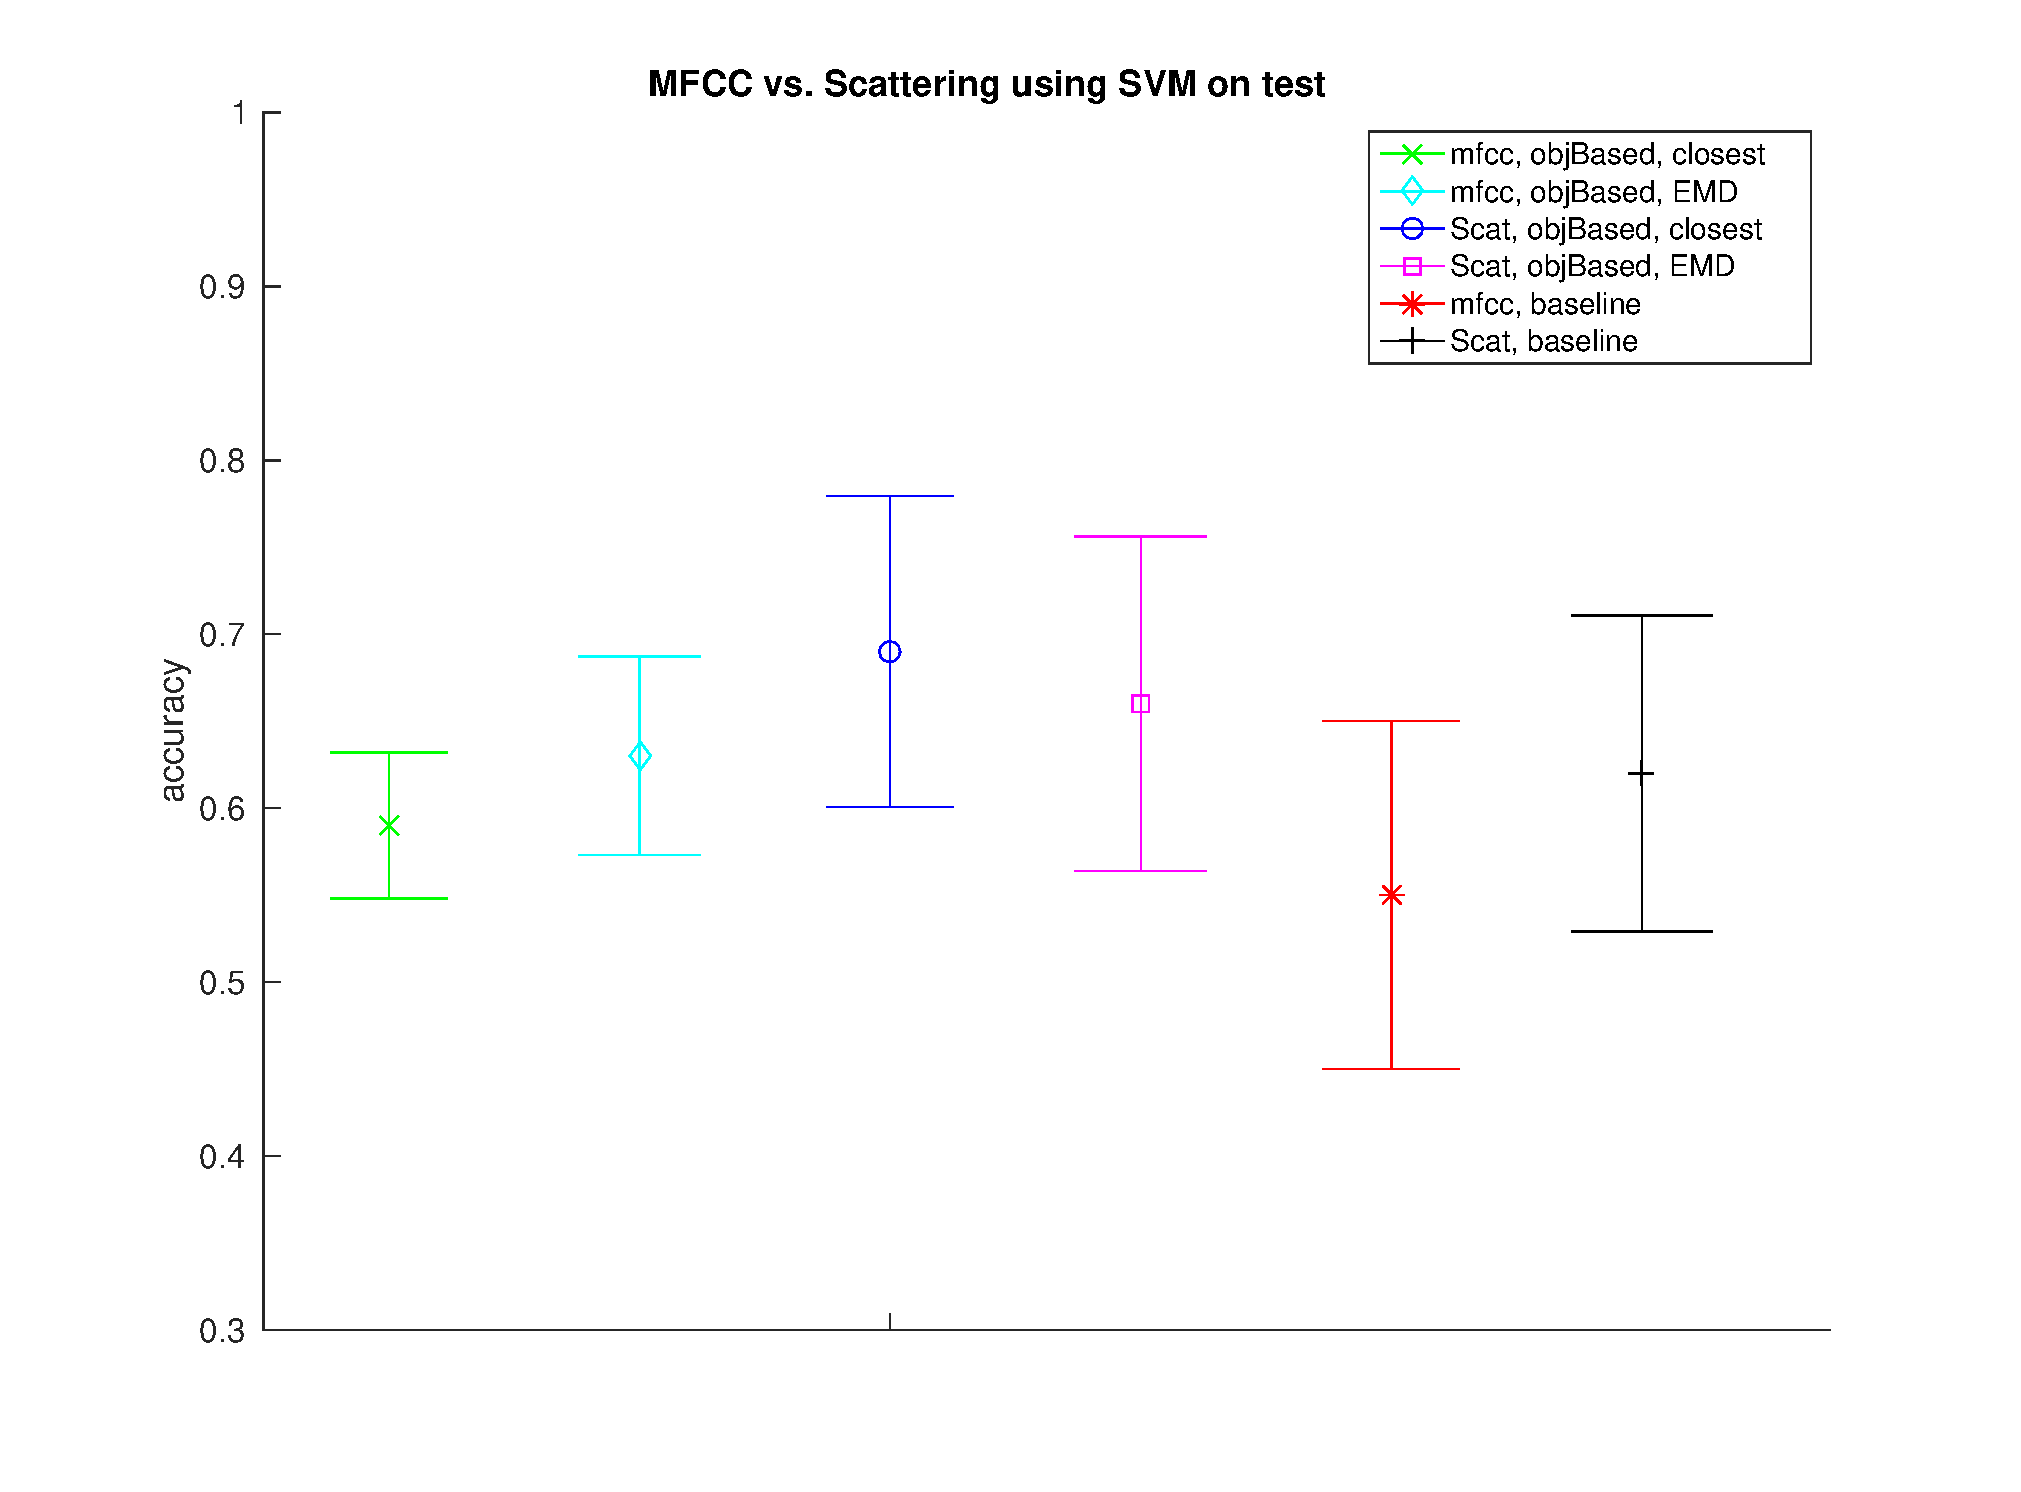
\includegraphics[width=\textwidth,height=0.8\textheight,keepaspectratio]{./figures/Fig6.pdf} 
\caption{cut: 0.02, set: test, select: 20} 
\label{cut0.02SetteSel20} 
\end{figure} 
\end{center} 
  
  
 % expLanesInsertionFlag DO NOT CLEAR (but move it where you want the generated temporary LaTEX code to be inserted) 
 
 
\bibliographystyle{abbrvnat}     
\bibliography{bib}     
 
\end{document}     
